% Finished September 26, 2013
% Put into VUW Thesis format Wednesday 2 April 2014

\documentclass[12pt, a4paper, twoside, openright]{book}

\usepackage{vuwthesis} % sets up some local things, mostly the front page

\setlength{\intextsep}{12pt} % set space above and below in-line float
\setlength{\abovecaptionskip}{0pt} % set space between figure and caption.


\usepackage{amssymb, amsmath}
%\usepackage{mathtools}
\usepackage{tikz}
\usetikzlibrary{calc}
\usepackage{url}

%\usepackage{marvosym}

\newcommand{\beff}{\ensuremath{b_{\mathrm{eff}}}}
\newcommand{\bmin}{\ensuremath{b_{\mathrm{min}}}}
\newcommand{\bmax}{\ensuremath{b_{\mathrm{max}}}}
\newcommand{\bfar}{\ensuremath{b_{\mathrm{far}}}}

\newcommand{\Tr}{\ensuremath{T_{\mathrm{room}}}}

\newcommand{\Finc}{\ensuremath{F_{\mathrm{inc}}}}
\newcommand{\Fads}{\ensuremath{F_{\mathrm{ads}}}}
\newcommand{\Fdes}{\ensuremath{F_{\mathrm{des}}}}
\newcommand{\Fcat}{\ensuremath{F_{\mathrm{cat}}}}

\newcommand{\kcat}{\ensuremath{k_{\mathrm{cat}}}}

\title{Chapter 9: Analogues of Effective Slip}
\author{Nat Lund}


\begin{document}
\chapter{Analogues of Effective Slip}

We have found the effective slip length for Stokes flow over a periodic mixed-slip surface.  However, on a purely mathematical level we have shown that Laplace's equation with a particular boundary condition:
\begin{gather}
\nabla^2 u = f \\
u = b(x,y) \frac{\partial u}{\partial z}
\end{gather}
has solutions:
\begin{equation}
\beff = \left< \frac{1}{b} \right>^{-1} \text{   if   } L \ll \bmin, \qquad \text{and} \qquad
\beff = \left< b \right> \text{   if   } \bmin \ll L
\end{equation}
Where $b$ is some periodic function on the boundary with units of length and period $L$.

\vspace{1em}
This models our slip problem.  The obvious question is: what other physical systems does it model?  If we can find appropriate systems, then we automatically have a solution --- some analogue of effective slip length.

We shall investigate two such physical systems forthwith: a thermal insulation problem and a heterogeneous catalyst problem.


\section*{Thermal Insulation}

Consider an atypical New Zealand house: one with insulation in the roof.  A standard house has an angled roof situated above a flat ceiling, with a fairly large crawlspace in between.  The ceiling panels are attached to the underside of wooden beams known as rafters, which are spaced 600 mm apart.  It is traditional to devote several entire weekends to laying insulating material on top of the ceiling panels, in the gaps between the rafters.
Thus, above the warm living space of a house, is a heterogeneous insulator, comprising wood (the rafters), highly insulating material, and those air gaps that are left over because you couldn't be bothered cutting scatchy, unwieldy fibreglass batts to exactly the right size.

\begin{figure}[ht]
\centering
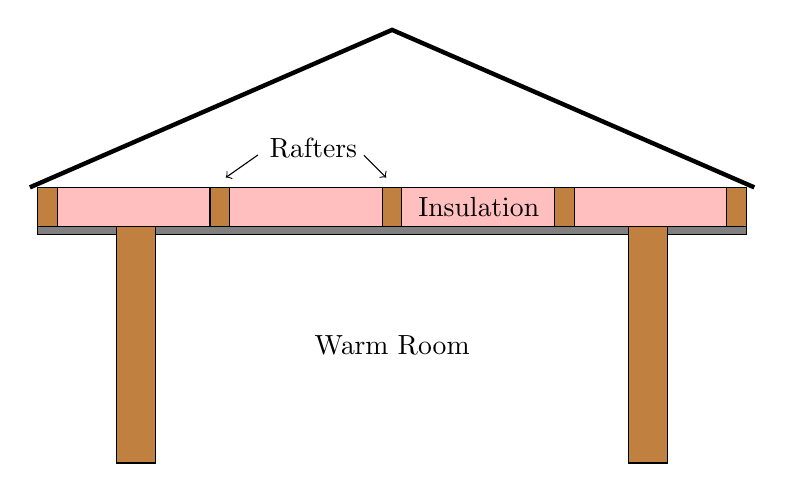
\begin{tikzpicture}
%Walls and ceiling
\draw[fill=brown] (0,0) rectangle ++(-0.5,-3);
\draw[fill=brown] (6,0) rectangle ++(0.5,-3);
\draw[fill=gray] (0,0) rectangle ++(6,-0.1);
\draw[fill=gray] (-1.5,0) rectangle ++(1,-0.1);
\draw[fill=gray] (6.5,0) rectangle ++(1,-0.1);

%Roof
\draw[fill=brown] (-1.5,0) rectangle ++(0.25,0.5);
\draw[fill=brown] (7.5,0) rectangle ++(-0.25,0.5);
\draw[ultra thick] (-1.6,0.5) -- ++(4.6,2) -- ++(4.6,-2);

% Rafters
\foreach \x in {1,2,3}
        {\draw[fill=brown] (-1.5,0) ++(\x*1.9375,0) ++(\x*0.25,0) rectangle ++(0.25,0.5);}

% Fibreglass batts
\foreach \x in {0,1,2,3}
        {\draw[fill=pink] (-1.25,0) ++(\x*1.9375,0) ++(\x*0.25,0) rectangle ++(1.9375,0.5);}

\node at (3,-1.5) {Warm Room};
\node at (2,1) {Rafters};
\draw[<-] (-1.25,0) ++(1.9375,0) ++(0.2,0.625) -- ++(35:0.5cm);
\draw[<-] (-1.25,0) ++(1.9375,0) ++(0.25,0) ++(1.9375,0) ++(0.05,0.625) -- ++(135:0.4cm);
\node at (4.1,0.25) {Insulation};

\end{tikzpicture}
\caption{a}\label{a}
\end{figure}

\subsection*{Mathematical Model}

We are interested in the `net' insulating properties of the heterogeneous insulator comprising wood, insulating material and possibly air gaps.  To that end, we model the heterogeneous insulator as a bulk material
with: a warm room at the lower boundary, and convection-dominated heat loss on the top boundary.  For consistency with our slip model, we shall invert the vertical dimension, and let $z=0$ denote the top of the bulk and $z=d$ the bottom of the bulk.  The temperature field is $T(x,y,z)$, with boundary conditions at $T(x,y,0)$ and $T(x,y,d)$, denoted $T(0)$ and $T(d)$.

\subsubsection*{Dirichlet Condition}

The warm room can be considered to be held at a constant temperature, due to the interventions of its human occupants.  Therefore, on the $z=d$ boundary is the Dirichlet condition
\begin{equation}
T(z) = \Tr = \text{constant}
\end{equation}

\subsubsection*{Bulk Condition}

The distribution of temperature $T$ in a material is governed by the diffusion equation:
\begin{equation}
\frac{\partial T}{\partial t} = \frac{k}{\rho C_p} \nabla^2 T
\end{equation}
where $k$ is the thermal conductivity, and $C_p$ is the specific heat capacity.

We shall assume that the system is at equilibrium, so that the time dependent term vanishes.  Hence, the solid material -- wooden rafters and insulating material -- is governed simply by Laplace's equation:
\begin{equation}
\nabla^2 T = 0
\end{equation}

\subsubsection*{Conductive Heat Current}
Consider a bar of test material of cross-sectional area $A$ clamped between a hot reservoir and a cold reservoir.
The heat current in the bar (Joules per second) depends on the temperature gradient, the thermal conductivity $k$ and the area $A$:
\begin{equation}
\frac{dQ}{dt} = k A \frac{\partial T}{\partial x}
\end{equation}

\begin{figure}[ht]
\centering
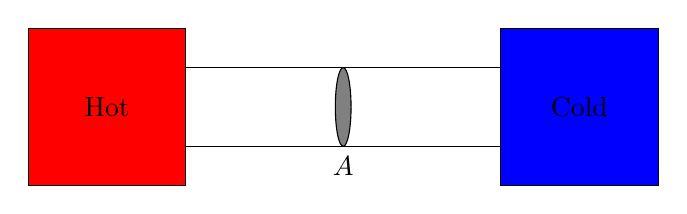
\begin{tikzpicture}
\draw[fill=red](0,-0.5) rectangle node{Hot} ++(-2,2);

\draw(0,0) rectangle ++(4,1);
\draw(0,0) ++(4,-0.5)[fill=blue] rectangle node{Cold} ++(2,2);

\draw (2,0.5)[fill=gray] ellipse (0.1cm and 0.5cm);
\node at (2,0) [below] {$A$};

\end{tikzpicture}
\caption{b}\label{b}
\end{figure}

\subsubsection*{Convective Heat Current}
Convection is harder to quantify than conduction.   
A plate at temperature $T$ convecting into an infinite reservoir of gas at temperature $T_0$ shows a heat flux approximately proportional to $(T - T_0)^{5/4}$.
However, consider the experimental setup in the diagram: a body of convecting air between a hot body and a cold body.  For such a system, the heat flux is usually considered to have a simple linear relationship to temperature difference. 

\begin{figure}[ht]
\centering
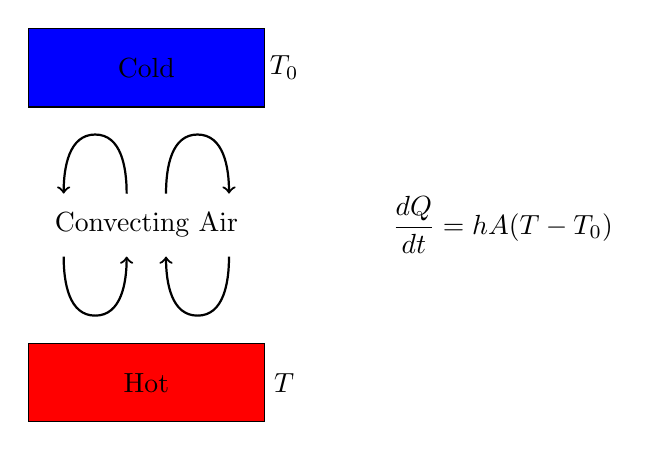
\begin{tikzpicture}
%\everymath{\displaystyle}

\node at (0,0) {Convecting Air};
\draw[fill=red] (-1.5,-1.5) rectangle node {Hot} ++(3,-1);
\draw[fill=blue] (-1.5,1.5) rectangle node {Cold} ++(3,1);

\node at (3,0)[right] {$\displaystyle \frac{dQ}{dt} = h A (T - T_0) $};

\node at (1.75,-2) {$T$};
\node at (1.75,2)  {$T_0$};

%Curved Arrows
\draw[->,thick] (0.25,0.4) to [out=90,in=180] ++(0.4,0.75) to [out=0,in=90] ++(0.4,-0.75);
\draw[->,thick] (-0.25,0.4) to [out=90,in=0] ++(-0.4,0.75) to [out=180,in=90] ++(-0.4,-0.75);
\draw[<-,thick] (0.25,-0.4) to [out=-90,in=180] ++(0.4,-0.75) to [out=0,in=-90] ++(0.4,0.75);
\draw[<-,thick] (-0.25,-0.4) to [out=-90,in=0] ++(-0.4,-0.75) to [out=180,in=-90] ++(-0.4,0.75);

\end{tikzpicture}
\caption{c}\label{c}
\end{figure}

This is known as Newton's law of cooling, and $h$ is the \emph{heat transfer coefficient.}

\subsubsection*{Convective Boundary Condition}

The highly-conductive steel roof of a house can be presumed to be at the same low temperature $T_0$ as the outside air. Then convection occurs between the bulk heterogeneous insulator and the cold roof, with heat flux \emph{leaving} the boundary given approximately by Newton's law of cooling.

Furthermore, heat flux will arrive \emph{at} the boundary in accordance with the heat conduction equation.

\begin{figure}[ht]
\centering
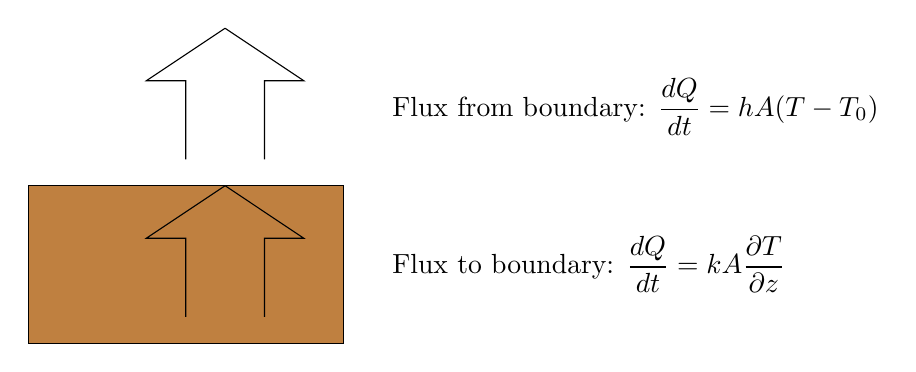
\begin{tikzpicture}
\draw[fill = brown] (1.5,0) rectangle ++(-4,-2);
\draw (0,0) -- ++(1,-0.667) -- ++(-0.5,0) -- ++(0,-1);
\draw (0,0) -- ++(-1,-0.667) -- ++(0.5,0) -- ++(0,-1);
\draw (0,2) -- ++(1,-0.667) -- ++(-0.5,0) -- ++(0,-1);
\draw (0,2) -- ++(-1,-0.667) -- ++(0.5,0) -- ++(0,-1);

\node at (2,-1)[right] {Flux to boundary: $\displaystyle \frac{dQ}{dt} = k A \frac{\partial T}{\partial z} $};
\node at (2,1) [right] {Flux from boundary: $\displaystyle \frac{dQ}{dt} = h A (T - T_0)$};

\end{tikzpicture}
\caption{d}\label{d}
\end{figure}

Since the boundary is a virtual plane with no heat capacity, the fluxes are always equal:
\begin{equation}
h A (T - T_0) = k A \frac{\partial T}{\partial z}
\end{equation}

For convenience, define the low temperature to be $T_0 = 0$.  Then the convective boundary condition is:
\begin{equation}
T = \frac{k}{h} \frac{\partial T}{\partial z}
\end{equation}

Now the heat transfer coefficient $h$ is constant for the system.  But the thermal conductivity $k$ varies spatiallly because the bulk material is heterogenous.  Therefore define the variable:
\begin{equation}
b(x,y) = \frac{k}{h}
\end{equation}

And we now have a system of equations equivalent to those describing steady shear-driven Stokes flow with Navier slip:
\begin{gather}
\nabla^2 T = 0 \\
T = b \frac{\partial T}{\partial z}
\end{gather}

The function $b(x,y)$ has units of length, and we can now solve to find an effective `insulation length' for the heterogeneous insulation.  To minimize heat loss for a given room temperature, we want the lowest temperature on the convective boundary, which in turn demands the lowest effective insulation length.

\begin{figure}[ht]
\centering
\begin{tikzpicture}
\draw [<->] (0,4) -- (0,0) -- (9,0);
\draw (4,0) -- ++(0,4);
\draw[thick, color=red] (0,3) -- (4,1.5);
\draw[thick, color=red,dashed] (4,1.5) -- (8,0);

\node at (4,0)[below] {0};
\node at (0,0)[below] {$d$};

\draw (0,3) -- ++(-0.1,0);
\node at (-0.1,3)[left] {\Tr};

\draw[<->] (4,-0.7) -- node[below]{\beff} ++(4,0);

\end{tikzpicture}
\caption{e}\label{e}
\end{figure}


\subsubsection*{Ready-Made Solution}

To apply one of the two solutions we have already found, we need to know which regime the system is in.

The heterogeneity of the bulk material is due to the wooden rafters, spaced about half a meter apart.  Thus the period $L \simeq 1$m.
The heat transfer coefficient for air is experimentally determined to be in the range 10 - 100 Wm$^{-2}$K${-1}$.

The thermal conductivity for wood depends on the moisture content: from 0.04 - 0-.12 Wm$^{-1}$K$^{-1}$ for oven-dry wood, and up to 0.4 Wm$^{-1}$K$^{-1}$ for wood with more than 12\% water content.
Typical highly-insulating materials might be polystyrene foam or polyurethane foam, with $k$ = 0.03 Wm$^{-1}$K$^{-1}$, or mineral wool, sheep's wool, or fibreglass wool, at $k$ = 0.04 Wm$^{-1}$K$^{-1}$.
Air itself -- if sufficiently constrained to avoid convection -- has a very low thermal conductivity of $k$ = 0.024 Wm$^{-1}$K$^{-1}$.

Thus values of $b = k/h$ are in the range 0.0003 to 0.012 meters.  Clearly, $b \ll L$ so we are in the regime where the effective insulation length is given by the area-weighted average:
\begin{equation}
\beff = \left< b \right>
\end{equation}


\vspace{1em}
Note that while the boundary condition is heterogeneous -- $b(x,y)$ is a function of position on the boundary plane -- this is due to the fact that \emph{bulk} is heterogeneous.  The coupling occurs because the heat fluxes match at the boundary.

\vspace{1em}
An interesting historical note: The first expression for effective slip is the one by J.R. Philip from 1972.  His method `generalizes a device of Karush and Young'.  The 1952 paper by Karush and Young
dealt with the effect of a periodic array of perfectly insulating stripes or circles, that partially block the loss of heat from a lump of radioactive material.


\section*{Catalysis}

One particularly widespread application of catalysts is in the catalytic converters fitted to the exhaust systems of motorcars.  Efforts are underway to improve these catalysts by the use of nanostructured material.  The improvement is partly from the increased surface area, and partly from a geometric effect: the sharp corners of a catalyst nanoparticle seem to be more active than flat surfaces of the same catalyst.

Thus, it is possible that a nanostructured catalyst has a catalytic activity that varies across a nominal surface  -- the catalyst is heterogeneous, and may be a candidate for modelling as a homogenization problem.  We shall attempt this here.

\vspace*{1em}
Below is a schematic diagram of a catalyst in action.  We shall consider the simplest case of a single gas species -- say N$_2$O$_4$, that diffuses to the surface of the catalyst, where a catalysed reaction breaks the molecule down into separate N$_2$ and O$_2$ molecules.  The catalyst surface has some `sharp bits' that have greater catalytic activity than the flat regions.



\begin{figure}[ht]
\centering
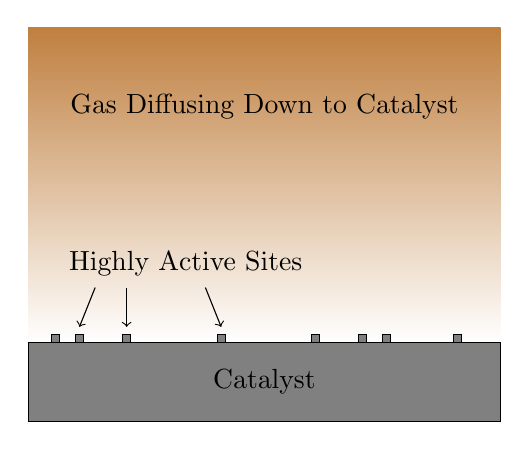
\begin{tikzpicture}

\shade[top color=brown] (0,0) rectangle ++(6,4);
\draw[fill=gray] (0,0) rectangle node {Catalyst} ++(6,-1);

\foreach \x in {0.5,1,2, 4, 6,7,7.5, 9}
                      {
                      \draw[fill=gray]  (6* \x/10, 0) rectangle ++(0.1,0.1);
                      }
 
\node at (2,1) {Highly Active Sites};
\draw[<-] (0.65,0.2) -- ++(0.2,0.5);
\draw[<-] (1.25,0.2) -- ++(0.0,0.5);
\draw[<-] (2.45,0.2) -- ++(-0.2,0.5);

\node at (3,3) {Gas Diffusing Down to Catalyst};


\end{tikzpicture}
\caption{f}\label{f}
\end{figure}

\subsubsection*{Model}

The concentration of the gas species (eg. N$_2$O$_4$) is $C$.  The presence of the reaction products is presumed to not influence the behaviour of the gas species, so they are ignored.
\vspace*{1em}

The system is `driven' by a fixed concentration of gas in the exhaust gases flowing past.  This gives the top boundary condition as $C(top) = C_D$.


\subsubsection*{Bulk Condition: Laplace}

Oxides of nitrogen comprise less than 1\% of exhaust gas, so our gas species is very dilute, and so its concentration is governed by the diffusion equation.  Furthermore, we shall assume equilibrium conditions, so the time-dependent term vanishes, and the bulk gas obeys Laplace's equation:
\begin{equation}
\nabla^2 C = 0
\end{equation}


\subsubsection*{Boundary Layer}

The layer of gas from which atoms rain down onto the surface is the \textbf{boundary layer}.  There are four fluxes of molecules associated with the boundary layer: the flux of particles \emph{into} the boundary layer from the bulk gas; the flux of particles that adsorb to the surface; the flux of particles that desorb from the surface before being catalysed; and the virtual flux of molecules destroyed by the catalyst, that leave the boundary layer by ceasing to exist. 

\begin{figure}[ht]
\centering
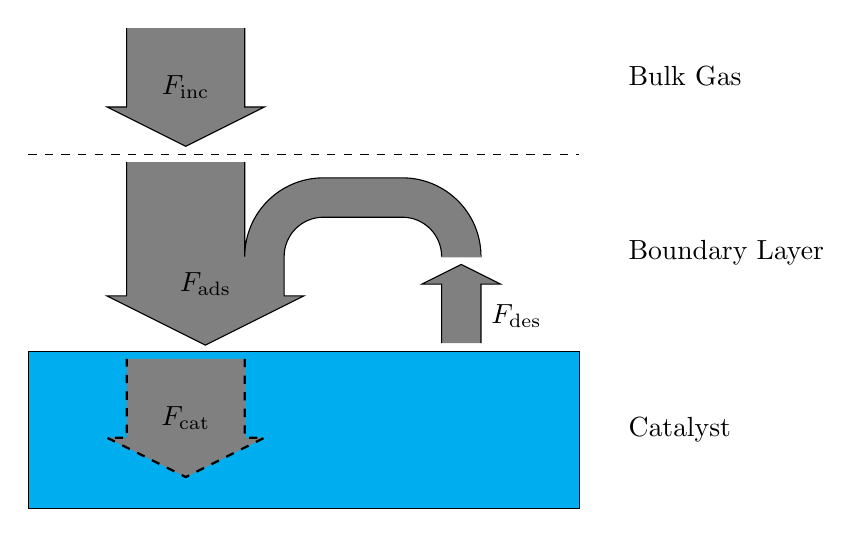
\begin{tikzpicture}
\draw[fill=cyan] (0,0) rectangle (7,-2);
\draw[dashed] (0,2.5) -- ++(7,0);

\node at (7.5,3.5)[right] {Bulk Gas};
\node at (7.5,1.25)[right] {Boundary Layer};
\node at (7.5,-1)[right] {Catalyst};

\coordinate (finc) at (2,2.6);
\draw[fill=gray] (finc) ++(0.75,1.5) -- ++(0,-1) -- ++(0.25,0) -- (finc) -- ++(-1,0.5) -- ++(0.25,0) -- ++(0,1);

\coordinate (fcat) at (2,-1.6);
\draw[thick,dashed, fill=gray] (fcat) ++(0.75,1.5) -- ++(0,-1) -- ++(0.25,0) -- (fcat) -- ++(-1,0.5) -- ++(0.25,0) -- ++(0,1);

\coordinate (fads) at (1.25,2.4);
\draw[fill=gray] (fads) -- ++(0,-1.7) -- ++(-0.25,0) -- ++(1.25,-0.625) -- ++(1.25,0.625)
-- ++(-0.25,0) -- ++(0,0.5) to [out=90,in=180] ++(0.5,0.5) -- ++(1,0)
to [out=0,in=90] ++(0.5,-0.5) -- ++(0.5,0) to [out=90,in=0] ++(-1,1) -- ++(-1,0)
to [out=180,in=90] ++(-1,-1) -- ++(0,1.2);

\draw[color=gray,fill=gray] (fads) ++(4,-1.2) -- ++(0.5,0) -- ++(-0.25,0.25);

\coordinate (fdes) at (5.25,0.1);
\draw[fill=gray] (fdes) -- ++(0,0.75) -- ++(-0.25,0) -- ++(0.5,0.25) -- ++(0.5,-0.25) -- ++(-0.25,0) -- ++(0,-0.75);


\node at (2,3.35) {\Finc};
\node at (2,-0.85) {\Fcat};
\node at (2.25,0.85) {\Fads};
\node at (6.2,0.45) {\Fdes};

\end{tikzpicture}
\caption{g}\label{g}
\end{figure}


\subsubsection*{Mass Balance}
There is a \emph{net} flux $\Finc$ of molecules per second entering the boundary layer.  There is a virtual flux of molecules destroyed per second by the catalyst, $\Fcat$.  By conservation of mass, they must be equal:
\begin{equation}
\Finc = \Fcat
\end{equation}

As an aside, there may also be an auxiliary flux cycle:
In order to be catalysed, a molecule must first adsorb to the catalyst.  However, in principle, an adsorbed molecule may \emph{desorb} before being catalysed.  Thus:
\begin{equation}
\Fads = \Fcat + \Fdes
\end{equation}


\subsubsection*{Incoming Flux}

The flux of molecules entering the boundary layer -- moles per second per square meter -- is given by Fick's first law of diffusion:
\begin{equation}
\Finc = D \frac{\partial C}{\partial z}
\end{equation}
For an ideal gas, the diffusion coefficient $D$ is given by $\frac{1}{3} \lambda \bar{u}$, where $\lambda$ is the mean free path in the gas and $\bar{u}$ is the mean speed of gas particles. So:
\begin{equation}
\Finc = \frac{1}{3} \lambda \bar{u} \frac{\partial C}{\partial z}
\end{equation}

\subsubsection*{Catalyzed Flux}

One can imagine how the behaviour of a catalyst could be studied experimentally.  Keeping temperature and pressure constant, for a given concentration of gas at the catalyst surface, the experimentalist will observe a certain number of moles catalysed per second (per square meter).  If the concentration is not too high, then we would expect the catalyzed flux to have a linear dependence on concentration.  (At higher concentrations, the catalyst will saturate.)
\begin{equation}
\Fcat \propto C 
\end{equation}

We can refine this with some statistical mechanics.  In Appendix A, we show that the flux incident on a surface in a gas of concentration $C$ is:
\begin{equation}
F = \frac{1}{4} \bar{u} C
\end{equation}
An incident particle has some probability of adsorbing to the surface, and once adsorbed has some probability of being catalysed before desorbing.  Let $\kcat$ be the probability that a particle striking the surface is adsorbed \emph{and} catalysed.  Then the virtual flux of particles hitting the surface and being catalysed out of existence is:
\begin{equation}
\Fcat = \frac{1}{4} \kcat \bar{u} C
\end{equation}

(If the concentration is very high, and the `dwell time' between adsorbing and vanishing is too long, then a pool of reactants will build up on the surface.  At some level of coverage, there is a non-negligible chance that an incident particle will bounce off an adsorbed particle, rather than striking the catalyst.  In these saturated conditions, the linear relationship will break down; put another way, $\kcat$ stops being a constant and becomes a function of $C$.)


\subsubsection*{Catalyst Boundary Condition}

As noted, by mass balance, $\Finc = \Fcat$. Therefore:
\begin{equation}
\frac{1}{3} \lambda \bar{u} \frac{\partial C}{\partial z} = \frac{1}{4} \kcat \bar{u} C
\end{equation}
Let us introduce the catalytic parameter:
\begin{equation}
b = \frac{4}{3} \frac{\lambda}{\kcat}
\end{equation}
Then the catalyst boundary condition is:
\begin{equation}
C = b \frac{\partial C}{\partial z}
\end{equation}
which once again resembles the Navier slip condition.
Furthermore, $b$ again has units of length, since it is a multiple of the mean free path.

If the catalyst is heterogeneous, perhaps due to nanostructure, then the catalytic parameter $b(x,y)$ is a function on the surface of the catalyst.

\vspace*{1em}




\subsection*{Solution}
We can provide a ready-made solution to
\begin{gather}
\nabla^2 C = 0 \\
C = b \frac{\partial C}{\partial z}
\end{gather}
provided that we know $b(x,y)$ as a function of position on the catalyst surface. Whether or not that is feasible is a question for chemistry, and is beyond the scope of this thesis.  This naive, physicist's analysis suggest that if it is feasible, then the homogenization technique may be applied, and an effective parameter for catalytic activity $\beff$ can be calculated.

\vspace*{1em}
Since $\kcat$ is a probability between 0 and 1, $b$ is in the range $\frac{4}{3}\lambda$ to $\infty$. The mean free path of air at standard temperature and pressure is $\lambda = 68$nm.  However temperatures and pressures in automotive catalytic converters are much higher: they need a temperature of at least 250$^{\circ}$C to work properly, and actual operating temperatures vary from 300$^{\circ}$C at idle up to 1000$^{\circ}$C if driven by bogans. Now,
\begin{equation}
\lambda = \frac{k_{\mathrm{B}} T}{\sqrt{2} \pi d^2 p}
\end{equation}
So, if typical $T$ is double or triple room temperature, and $p$ is somewhat higher than ambient, then we would expect $\lambda \sim 100$nm, and similarly $b \geq 100$nm.

The appropriate solution regime depends on $L$ and $\kcat$.  If a `nanostructured' catalyst truly has a roughness with a period of at most tens of nanometers, then certainly $L \ll b$, regardless of $\kcat$, so that:
\begin{equation}
\beff = \left< \frac{1}{b} \right>^{-1} \quad \text{if} \quad L < \sim 100 \mathrm{nm}
\end{equation}

If on the other hand, the surface structure has a period of a micron or more, and the catalyst is reasonably efficient -- $\kcat > \sim 0.5$ -- then $b \ll L$ and:
\begin{equation}
\beff = \left< b \right> \quad \text{if} \quad L > \sim 1 \mu \mathrm{m} \;\;\; \text{and} \;\;\; \kcat > \sim 0.5
\end{equation}

If the catalyst is very inefficient, $\kcat < 0.1$, then $b$ is very sensitive to small changes in $\kcat$.  Therefore we cannot give any definite guidelines about whether the system is in the $b \ll L$ regime or the $L\ll b$ regime.

\vspace*{1em}
Conversely, if the effective catalytic activity of a nanostuctured catalyst is measured, and compared with the standard flat plane morphology, then the activity of the sharp bits of the catalyst may be estimated using the homogenized harmonic mean (or mean) formula.

\end{document}
